% title: Scaled dot-product and multi-head attention
% description: Two panels: scaled dot-product attention (MatMul, Scale, optional Mask, Softmax, MatMul) and multi-head attention (h stacked Linear projections and attention heads, Concat, Linear), with the attention equation.
\documentclass[tikz,border=10pt]{standalone}
\usepackage{amsmath}
\usetikzlibrary{arrows.meta,positioning,fit,backgrounds,calc,shadows}

\definecolor{mat}{HTML}{D9D0F0}
\definecolor{scale}{HTML}{F3EFAE}
\definecolor{mask}{HTML}{F7C6D2}
\definecolor{soft}{HTML}{CBEACF}
\definecolor{lin}{HTML}{C6E5F7}
\definecolor{attn}{HTML}{FCE0BE}
\definecolor{cat}{HTML}{F3EFAE}

\tikzset{
  every node/.style={font=\sffamily\small},
  op/.style={draw, rounded corners=3pt, minimum width=24mm, minimum height=7mm, align=center,
    line width=0.6pt},
  stacked/.style={double copy shadow={shadow xshift=1.3mm, shadow yshift=1.3mm, fill=#1,
    draw}, fill=#1},
  flow/.style={-{Stealth[length=2.2mm]}, line width=0.7pt, rounded corners=3pt},
  panel/.style={font=\sffamily\bfseries},
}

\begin{document}
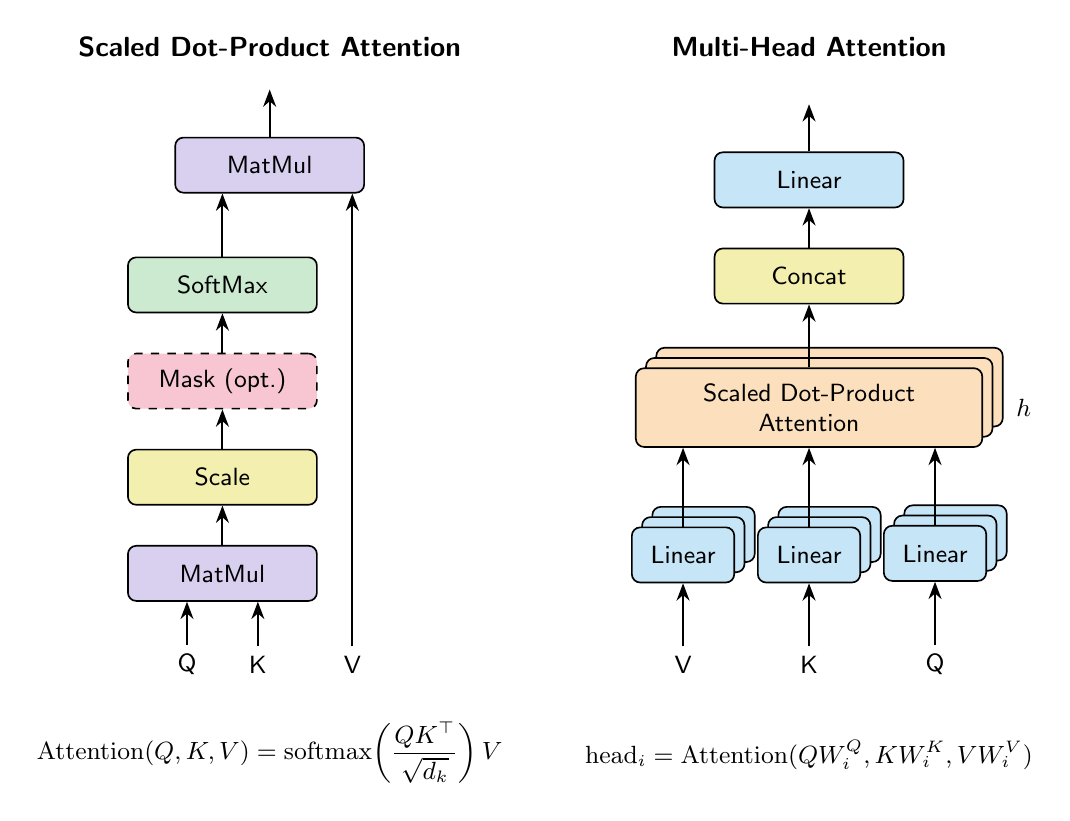
\begin{tikzpicture}

% ---------------- Scaled dot-product attention ----------------
\node (q) at (-9mm,0) {Q};
\node (k) at (0mm,0) {K};
\node (v) at (12mm,0) {V};
\node[op, fill=mat, above=8mm of $(q)!0.5!(k)$] (mm1) {MatMul};
\node[op, fill=scale, above=5mm of mm1] (sc) {Scale};
\node[op, fill=mask, above=5mm of sc, dashed] (mk) {Mask (opt.)};
\node[op, fill=soft, above=5mm of mk] (sm) {SoftMax};
\node[op, fill=mat, above=8mm of sm, xshift=6mm] (mm2) {MatMul};

\draw[flow] (q) -- (q |- mm1.south);
\draw[flow] (k) -- (k |- mm1.south);
\draw[flow] (mm1) -- (sc);
\draw[flow] (sc) -- (mk);
\draw[flow] (mk) -- (sm);
\draw[flow] (sm.north) |- ++(0,3mm) -| ($(mm2.south)+(-6mm,0)$);
\draw[flow] (v) -- (v |- mm2.south);
\draw[flow] (mm2.north) -- ++(0,6mm);

\node[panel, above=9mm of mm2] (t1) {Scaled Dot-Product Attention};
\node[below=6mm of $(q)!0.5!(v)$] {$\operatorname{Attention}(Q,K,V)=\operatorname{softmax}\!\left(\dfrac{QK^{\top}}{\sqrt{d_k}}\right)V$};

% ---------------- Multi-head attention ----------------
\begin{scope}[xshift=70mm]
  \node (hv) at (-16mm,0) {V};
  \node (hk) at (0mm,0) {K};
  \node (hq) at (16mm,0) {Q};
  \foreach \n in {hv, hk, hq} {
    \node[op, stacked=lin, minimum width=13mm, above=8mm of \n] (l\n) {Linear};
    \draw[flow] (\n) -- (l\n);
  }
  \node[op, stacked=attn, minimum width=44mm, minimum height=10mm, above=10mm of lhk] (sdpa)
    {Scaled Dot-Product\\Attention};
  \foreach \n in {hv, hk, hq} {
    \draw[flow] (l\n) -- (l\n |- sdpa.south);
  }
  \node[right=3mm of sdpa.east] {$h$};
  \node[op, fill=cat, above=8mm of sdpa] (cat) {Concat};
  \node[op, fill=lin, above=5mm of cat] (out) {Linear};
  \draw[flow] (sdpa) -- (cat);
  \draw[flow] (cat) -- (out);
  \draw[flow] (out.north) -- ++(0,6mm);
  \node[panel] at (t1 -| sdpa) {Multi-Head Attention};
  \node[below=6mm of hk] {$\operatorname{head}_i=\operatorname{Attention}(QW_i^{Q},KW_i^{K},VW_i^{V})$};
\end{scope}

\end{tikzpicture}
\end{document}
